% !TEX root = ../swputhesis.tex
\chapter{绪论}
\section{研究背景与意义}
随着信息技术和互联网的迅猛发展，网络已经深度融入社会运行与人
民生活的各个方面，成为支撑经济发展、社会治理和公共服务的重要
基础设施。教育、金融、医疗、政务、工业互联网等关键领域对网络
的依赖程度不断提高，网络空间已成为国家安全和社会稳定的重要组
成部分。与此同时，网络规模持续扩大，网络流量呈现出高速增长、
多样化和高度动态化的特征，使网络运行环境日益复杂。根据中国互
联网络信息中心（CNNIC）发布的统计数据\cite{CNNIC2025}，我国网民规模和互联网
普及率持续攀升，如图\ref{fig:11}所示，网络基础设施和在线应用的快速发展带来了海量数
据交换和频繁的业务交互，为网络流量分析与管理提出了更高要求。

\begin{figure}[h]
	\centering
	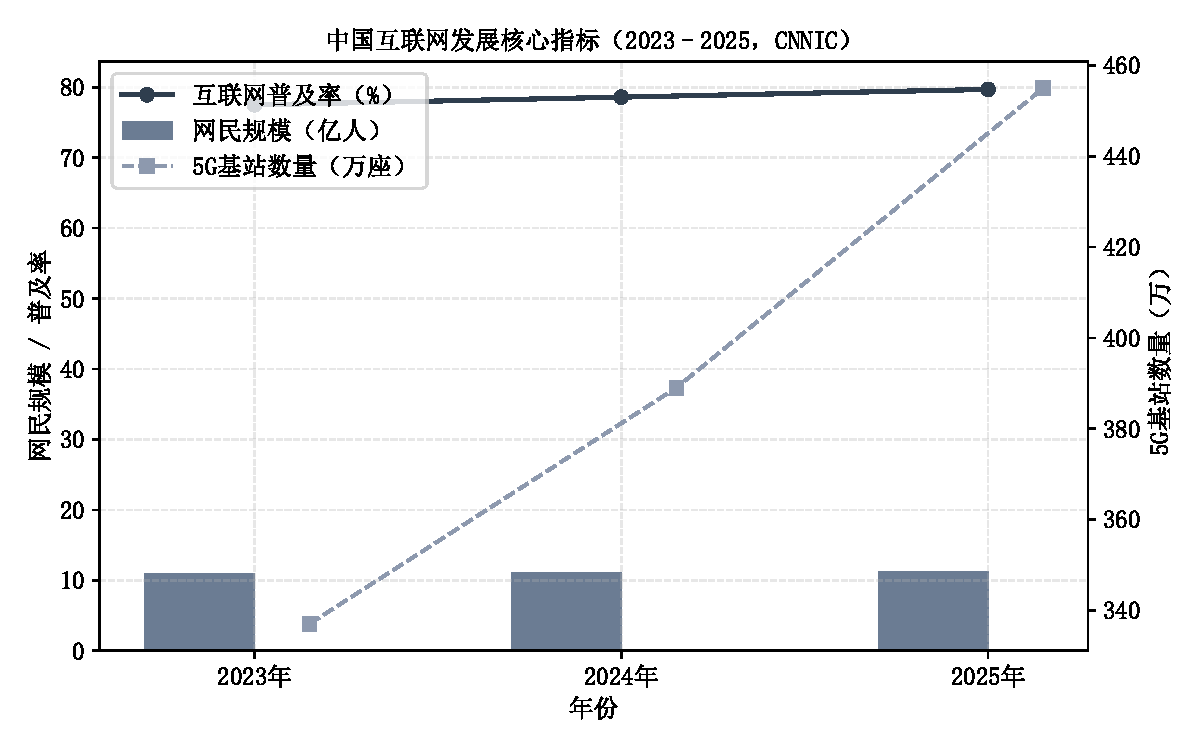
\includegraphics[scale=0.6]{fig/chapter1/cnnic_2025_trend.pdf}
	\caption{中国网民规模和互联网普及率（2023–2025年）}
	\label{fig:11}
\end{figure}

在网络快速发展的同时，网络安全威胁也呈现出数量激增和形态演化
的趋势。传统以单点漏洞利用为主的攻击方式逐渐向多阶段、跨平台
、隐蔽性强的高级持续性威胁（APT）演进，分布式拒绝服务攻击（
DDoS）、供应链攻击、恶意软件传播和针对关键基础设施的定向攻击
频繁发生。这类攻击往往通过异常的连接行为、突发流量、通信模式
变化或持续性隐蔽通信体现出来，对金融系统、能源系统、交通系统
和政务网络造成严重威胁。网络攻击不仅会导致网络服务中断和经济
损失，还可能引发社会秩序和国家安全风险，因此对网络异常行为的
及时识别与预警已成为网络安全防护体系中的核心任务。

网络流量作为用户通信行为和网络运行状态的直接反映，是发现安全威
胁和异常行为的重要数据基础。通过对流量特征、时序变化和通信模式
的分析，可以揭示网络中潜在的攻击活动、异常访问和资源滥用现象。
异常网络流量检测技术因此成为入侵检测系统、态势感知平台和网络安
全运维的重要组成部分。然而，随着网络规模的扩大和应用类型的多样
化，传统基于规则匹配和特征签名的检测方法逐渐暴露出局限性。这类
方法高度依赖人工构建的规则库和已知攻击特征，对未知攻击和变种攻
击的适应能力不足，在高维、大规模和高速流量环境中还面临着实时性
和可扩展性问题。与此同时，加密流量比例的不断上升使得基于内容特
征和载荷分析的传统检测手段进一步受限，仅依靠协议字段和浅层特征
已难以有效刻画复杂的通信行为。

在实际网络环境中，大规模流量数据往往缺乏精确标注，异常样本稀少
且分布不均，这使得依赖标签数据的监督学习方法在训练成本、模型泛
化能力和实际部署方面受到制约。相比之下，无监督学习方法能够在无
需人工标注的条件下，从大量未标注流量中自动学习正常通信行为的统
计规律和结构特征，并将偏离这些规律的流量识别为异常，在未知攻击
检测和动态网络环境中具有更强的适应能力。近年来，自编码器、聚类
方法、孤立森林以及基于深度表示学习的无监督模型在异常检测领域取
得了显著进展，为复杂网络流量建模和异常识别提供了新的技术路径。

同时，准确可靠的异常流量检测技术对于网络资源调度、负载均衡和服
务质量保障也具有重要意义。通过对异常流量的实时发现与预警，可以
有效避免网络拥塞、服务中断和性能下降，为网络运维与安全管理提供
科学依据。更进一步，随着数字经济、工业互联网和智慧城市建设的不
断推进，构建高效、自适应的异常网络流量检测体系，对于保障关键信
息基础设施安全、维护国家网络空间安全和支撑社会数字化运行具有重
要的战略价值。

在此背景下，开展基于无监督学习的异常网络流量检测研究，不仅有助
于突破传统规则驱动和监督学习方法在复杂网络环境中的局限，而且能
够有效应对标签匮乏、攻击多样化和加密流量普及等现实挑战。通过对
网络流量的时序特征、统计特性和行为模式进行深层次建模，可以在无
需依赖已知攻击样本的情况下发现潜在威胁，提高对新型攻击、变种攻
击和隐蔽通信的检测能力，从而提升网络安全防护的智能化和自动化水
平。在复杂真实网络环境中，异常网络流量检测面临着若干关键技术瓶
颈，其中尤以异常样本稀缺和未知攻击难以识别最为突出。

（1）异常样本稀少且标注困难的问题。在实际网络运行过程中，绝大多
数流量属于正常业务通信，而异常流量通常只在攻击发生或系统异常时短
暂出现，具有低发生率和强不平衡性的特点。此外，异常流量的精确标注
往往依赖于安全专家对网络日志、流量行为和攻击过程的综合分析，不仅
人工成本高，而且在加密通信和复杂业务环境下难以保证标注的一致性与
准确性。这使得大规模、高质量的标注异常流量数据难以获得，导致基于
监督学习的检测方法在训练阶段容易出现过拟合或泛化能力不足的问题，
难以适应真实网络环境中不断变化的流量分布。

（2）未知攻击与变种攻击难以有效检测的问题。现有多数异常流量检测
和入侵检测方法依赖于历史攻击样本或预定义特征规则，对已知攻击类型
具有较好的识别能力，但当攻击者采用新的攻击手段、变更攻击特征或利
用零日漏洞时，这类方法往往失效。随着APT攻击、分布式协同攻击和隐
蔽通信技术的不断发展，攻击行为呈现出低频化、持续化和高度隐蔽的特
征，仅基于已知样本或静态规则构建的模型难以准确刻画其行为模式，容
易造成漏报和误报，从而削弱网络安全防御体系的有效性。

正是在上述两方面挑战的共同作用下，基于无监督学习的异常网络流量检
测方法逐渐成为研究热点。无监督学习无需依赖人工标注的异常样本，而
是通过对大量正常网络流量的统计特征和时序行为进行建模，自动学习正
常通信模式的内在分布结构，从而将偏离该分布的流量判定为异常。这种
以“正常行为建模”为核心的检测机制，使模型在面对异常样本稀缺和未知
攻击频繁出现的情况下仍具有较强的鲁棒性和泛化能力，能够更好地适应
复杂、动态和开放的网络环境。

综上所述，基于无监督学习的异常网络流量检测研究在理论上有助于推
动机器学习与网络安全领域的交叉融合，在技术上能够提升对未知威胁
的识别能力，在工程应用和国家安全层面则为构建智能化、可靠的网络
安全防御体系提供重要支撑，因此具有显著的学术意义和现实价值。

\section{国内外研究现状}
\subsection{异常流量检测研究现状}
随着互联网规模的不断扩大和网络应用场景的日益复杂，网络异常流量检测已
成为网络安全领域的重要研究方向。网络异常流量检测的核心目标是在海量网
络流量数据中及时、准确地识别异常或恶意行为，从而保障网络系统的安全与
稳定运行。从研究范式上看，异常流量检测通常被视为一种分类或异常识别问
题，其技术手段经历了由统计分析方法、传统机器学习方法向深度学习与集成
学习方法不断演进的发展过程。

早期的网络异常流量检测方法主要基于统计学原理，通过分析网络流量的统计
特征（如包大小、延迟、协议分布等）来识别异常行为。该类方法通常依赖于
对历史正常流量的建模，并通过设定阈值判断当前流量是否异常。典型研究如
基于置信度滤波、阈值判别及流量容量建模的方法，在检测DDoS攻击和蠕虫病
毒等显著异常行为方面取得了一定成效。统计方法计算简单、实现成本低，但
对复杂攻击和新型未知威胁的检测能力有限，且对阈值设定和历史数据依赖较
强，适应性不足。

网络异常流量检测逐渐向高维特征建模、时序关联学习和无监督检测方向发展。
相较于早期依赖人工特征和规则的方法，研究者更加关注模型对复杂攻击行为
和未知威胁的适应能力。在无监督异常检测方面，自编码器仍是研究热点之一
。Park等人提出面向网络数据包的无监督异常检测模型\cite{Park2025Unsupervised}，仅利用
正常流量进行训练，通过对抗训练降低模型对异常流量的重构能力。实验结果
表明，该方法在保持较高检测精度的同时，大幅减少模型参数量，具备较好的
实时检测潜力。然而，该类方法仍容易受到噪声特征和阈值设定的影响。

为进一步挖掘网络流量中的时序与空间特征，研究者开始将卷积神经网络与循
环神经网络进行融合。Mirsky 等人提出了基于自编码器的无监督网络入侵检
测系统 Kitsune\cite{Mirsky2018Kitsune}，该方法通过多层自编码器
对网络流量的正常行为进行建模，并利用重构误差实现异常检测。实验结果表明
，该模型在无需攻击标签的情况下，能够有效检测多种网络攻击行为，在多种真
实网络环境中表现出较高的检测准确率和良好的实时性。Lansky等人\cite{lansky2021deep}
对近年来深度学习入侵检测方法进行了系统评估，指出时空特征融合模型在复杂攻
击识别方面具有明显优势，但模型结构复杂、计算成本较高。

随着注意力机制的发展，Transformer模型逐渐被引入网络异常流量检测领域。
Shi等人\cite{Shi2022TransformerBiLSTM}将Transformer与BiLSTM相结合，实现全局特征建模与时
序依赖学习的协同优化，在不平衡数据场景下表现出更强的检测能力。Tuli 等人提出了一种基于Transformer
的无监督异常检测模型 TranAD\cite{tuli2022tranad}，该方法利用自注意力机制对时间序列数据进行建模
，能够有效捕捉网络流量中的长期依赖关系和关键特征模式。实验结果表明，Transformer结构在复杂时序异常
检测任务中具有较强的特征建模能力，为网络流量异常检测提供了新的建模思路。然而，此类模型通常对计算资源
依赖较强，限制了其在实际网络环境中的部署。

部分研究开始探索将图结构建模引入无监督异常检测任务中。Ding 等人提出了基于图自编码器的异常检测模型 
DOMINANT\cite{Ding2019DOMINANT}，通过联合建模节点属性与图结构信息，实现对异常节点的无监督检
测。实验结果表明，该方法在复杂关系数据中具有较好的检测性能和泛化能力，为将网络流量建模为图结构并开
展异常检测提供了有效思路。此外，Zerveas 等人提出了一种基于 Transformer 的自监督表示学习框架，
通过对多变量时间序列进行自监督训练，有效提升了模型在不同数据分布下的泛化能力\cite{Zerveas2021TransformerSSL}。
相关研究表明，将自监督学习与 Transformer 结构相结合，有助于缓解跨数据集场景中模型性能下降的问题，
该思想同样适用于网络入侵检测等复杂时序建模任务。

已有研究表明，基于自动化机器学习（AutoML）的数据驱动方法能够有效提升入侵与异常检测的性能。Xu 等人
提出了一种面向物联网环境的 AutoML 入侵检测方法，通过自动化模型选择与参数优化构建检测模型，在保证检
测准确率的同时增强了模型的鲁棒性与泛化能力\cite{xu2023data}。
Ozçelebi等对随机森林、XGBoost和LightGBM等方法在CIC-IDS-2017上进行了比较，发现集成模型在不平衡情况下表现出色
\cite{Ozcelebi2025EnsembleComparison}。在复杂场景中，注意力增强型LSTM与梯度提升类集成策略结合也被证明具有提升稀
有攻击检测能力的潜力\cite{SmartGrid2025Attentional}。此外，近期研究表明，通过将特征选择机制与集成学习框架相结合，
能够进一步提升入侵检测模型在不同数据集下的稳定性与泛化性能。Injadat 等人提出了一种融合混合特征选择与集成学习的入侵
检测方法，通过筛选关键特征并组合多种分类器，在多个基准数据集上验证了该方法在检测准确率和鲁棒性方面
的优势\cite{Injadat2023EnsembleFS}。

总体而言，当前网络异常流量检测研究已从基于规则和统计的方法逐步发展到
以机器学习、深度学习和集成学习为核心的智能检测阶段。尽管现有方法在检
测精度和适应性方面取得了显著进展，但在对未知攻击的鲁棒检测、异常样本
稀少、特征选择自动化以及模型复杂度控制等方面仍存在不足。因此，设计兼
顾检测性能、计算效率和泛化能力的异常流量检测方法，仍是该领域亟需深入
研究的重要方向。

\subsection{基于异常流量检测的机器学习方法}

基于异常流量的机器学习方法通过对网络流量数据进行建模与分析，实现对正常行为模式与异常行为模式的区分，
是当前网络安全领域中应用最为广泛的异常检测技术之一。该类方法通常以网络流量的统计特征、行为特征或时序
特征作为输入，通过机器学习算法对流量进行训练与判别，从而实现对异常流量的自动识别。根据是否依赖人工标
注数据以及模型结构的不同，基于异常流量的机器学习方法主要可分为有监督学习方法、无监督学习方法\cite{nassif2021machine}
以及基于深度学习的方法。 

（1）基于有监督学习的异常流量检测方法
有监督学习方法依赖于大量已标注的网络流量数据，通过学习正常流量与异常流量之间的差异，构建分类模型以实现
异常检测\cite{megantara2021hybrid}。常见的有监督学习算法包括支持向量机（Support Vector Machine，SVM）、决策树、随机森林、K
近邻算法以及朴素贝叶斯等。这类方法通常具有较高的检测精度和较强的判别能力，尤其在已知攻击类型和标签较为
完备的情况下，能够取得较为理想的检测效果。然而，在实际网络环境中，异常流量样本往往数量有限且标注成本较
高，容易导致数据集类别不平衡问题，从而影响模型的泛化能力。因此，有监督学习方法在应对未知攻击或新型异常
流量时存在一定局限性。

（2）基于无监督学习的异常流量检测方法
无监督学习方法不依赖人工标注数据，而是通过挖掘网络流量数据的内在结构和分布特征，自动识别偏离正常模式的
异常行为\cite{UnsupervisedReview2023}。该类方法通常假设正常流量在特征空间中具有较高的相似性，而异常流量则表现为离群点或低概率事件。
典型的无监督学习算法包括聚类算法（如K-means、层次聚类）、密度估计方法以及基于概率模型的方法（如高斯混
合模型）。无监督学习方法在异常标签稀缺的场景下具有较强的实用价值，能够有效发现未知异常模式，但其检测性
能在一定程度上依赖于特征选择和参数设置，且对复杂、高维流量数据的建模能力有限。

（3）基于深度学习的异常流量检测方法
随着大数据与深度学习技术的快速发展，基于深度学习的异常流量检测方法逐渐成为研究热点\cite{kim2020deep}。该类方法能够通过多
层非线性结构自动学习网络流量的高层特征表示，减少对人工特征工程的依赖。常见模型包括卷积神经网络（CNN）
、循环神经网络（RNN）、长短期记忆网络（LSTM）以及自编码器（Autoencoder，AE）等。其中，CNN在捕捉流
量空间特征方面具有优势，RNN及LSTM在处理时间序列流量数据、建模长期依赖关系方面表现突出，而自编码器则常
用于基于重构误差的无监督异常检测任务。近年来，生成对抗网络（GAN）及图神经网络（GNN）也逐渐被引入异常流
量检测领域，以提升模型对复杂网络结构和动态变化行为的建模能力。

总体而言，基于异常流量的机器学习方法在网络安全防护中发挥着重要作用。传统机器学习方法在特定场景下具有较
高的稳定性和可解释性，而深度学习方法在处理大规模、高维度和复杂时序流量数据方面展现出更强的表达能力。如
何在检测精度、计算复杂度与实际部署成本之间取得平衡，并提升模型对未知异常流量的检测能力，仍是该领域亟待
研究的重要问题。

\subsection{基于异常流量检测的深度学习方法}
随着网络环境的复杂化和网络攻击手段的不断演进，传统基于规则或浅层机器学习
的异常流量检测方法在特征表达能力和泛化性能方面逐渐暴露出局限性。深度学习
方法通过构建多层神经网络结构，能够自动从大规模网络流量数据中学习高层次、
非线性的特征表示，在异常流量检测领域展现出显著优势，已成为当前研究的主流方向之一。

早期研究主要集中于将基础神经网络结构引入异常流量检测任务。例如，Devan 
及其团队使用了前馈神经网络（Feedforward Neural Network, FNN）结合
XGBoost 特征选择方法，形成了XGBoost-FNN异常流量检测模型\cite{devan2020efficient}
，在NSL-KDD等经典数据集上取得了优于传统贝叶斯分类器和支持向量机的检测性能。同时，
Ghorbani 及其团队提出了一种基于稀疏自动编码器（Sparse Auto Encoder, SAE）
用于流量特征降维与表示学习\cite{ghorbani2022deep}，
其中SAE能够在减少特征冗余的同时保留关键判别信息，不仅提升了检测精度，
还有效降低了模型训练时间。实验结果表明，SAE 的效果优于基于随机森林和主成分分析的特征降维方法，
并且能够显著减少模型训练所需时间。

随着卷积神经网络（CNN）在图像领域取得突破性进展，此外，研究者提出了基于
网络流量图像可视化的分类方法，通过将流量数据转换为二维图像并利用机器学习
模型进行分类，从而实现对恶意流量的检测与分析。Demmesse 等人采用图像化方
式将网络流量表示为灰度图或彩色图，然后基于卷积神经网络等机器学习算法对这
些图像进行分类，有效提升了对隐匿性恶意流量的识别精度，展示了图像表示技术
在网络流量分类与异常检测中的潜力\cite{Demmesse2023ImageTraffic}。大
量实验表明，不同尺寸和构建方式的流量灰度图会对检测效果产生显著
影响，合理的图像表示有助于提升模型的识别能力，尤其在僵尸网络流量和加密流
量检测任务中表现突出。

针对网络流量天然具有时序特性的特点，循环神经网络（RNN）及其改进模型被广
泛应用于异常流量检测。RNN能够捕获流量数据中的时间依赖关系，但在处理长期
依赖问题时存在一定不足。因此，长短期记忆网络（LSTM）和门控循环单元（GRU
）逐渐成为主流选择。这类模型在NSL-KDD、UNSW-NB15等数据集上的实验结果表
明，其在二分类和多分类任务中均优于传统RNN模型，能够更准确地刻画复杂攻击行
为的时序特征。

随着单一深度学习模型在特征表达方面的局限性逐渐显现，研究者开始关注多模型融
合的异常流量检测方法。Khan 提出了 HCRNNIDS 模型\cite{khan2021hcrnnids}，
将 CNN 和 RNN结合为CRNN结构，使模型能够分别学习网络流量数据的空间特
征与时序关系，在 CICIDS2018 数据集上取得了 97.75\%的二分类准确率。该模型的性
能优于仅使用LSTM或CNN的模型，远超传统机器学习算法的对比模型。Wu等人设
计了ResBlk结构\cite{wu2020pelican}，将CNN和门控循环单元融合，并使用残差连接和批标准化技术，
在NSL-KDD 的 10折交叉验证任务中取得了 99.21\%的二分类准确率。Sinha等人\cite{sinha2020efficient}将
一维CNN和BiLSTM组成堆叠模型，在多个异常流量检测数据集上进行多分类实验，
实验结果显示，该堆叠模型的整体准确率和少数类别F1值均优于对比模型。

近年来，注意力机制的引入为异常流量检测提供了新的研究思路。通过在模型中引入
通道注意力、自注意力或多头注意力机制，可以对关键流量特征进行加权，从而提升
模型对重要信息的关注能力。Lan等研究者提出了MEMBER模型\cite{lan2022member}，该模型利用通道
注意力机制的卷积多任务学习，在多个流量异常检测领域基准数据集上取得了较高的
F1 值。Fu等研究者通过BiLSTM学习流量数据时序特征，并利用通道注意力影响特征
图，大量消融实验表明了通道注意力在异常流量检测上的有效性\cite{fu2022deep}。张安琳等研究者
使用自注意力机制对 CNN 和 BiGRU 提取的特征进行加权处理\cite{张安琳2022基于}，该方法在
CICIDS2018 数据集上的总精确率与召回率均得到提升。杨月麟等研究者提出了一种卷
积神经网络与Transformer结合的异常检测模型\cite{杨月麟2021基于深度学习的网络流量异常检测}，
并使用CReST类别再平衡算法解决数据集不平衡问题。在 CICIDS2017 数据集上实现了较高的准确率，
同时在 DoS 和Probe 等少数类别上的检测率与召回率优于对比模型。

随着深度学习方法的不断演进，越来越多研究将注意力机制、混合模型结构与自动学习能
力引入异常流量检测中，从而显著提升了检测精度与特征自动提取能力
\cite{hozouri2025comprehensive}，然而，这些方法在小样本条件下的训练效率与跨场景泛化能力仍然受到挑战。
 为此，研究者提出了结合自注意力机制的少样本入侵检测框架来增强模型鲁棒
 性与跨域适应能力\cite{xu2025few}，同时也有工作采用增量特征学
 习与相似性嵌入方法提升对未知攻击的实时检测能力\cite{alitbi2025generalized}。

\section{本文主要研究内容及创新}

\subsection{主要研究内容}
本论文主要研究内容包含三个部分，如图\ref{fig:13}所示。
\begin{figure}[h]
	\centering
	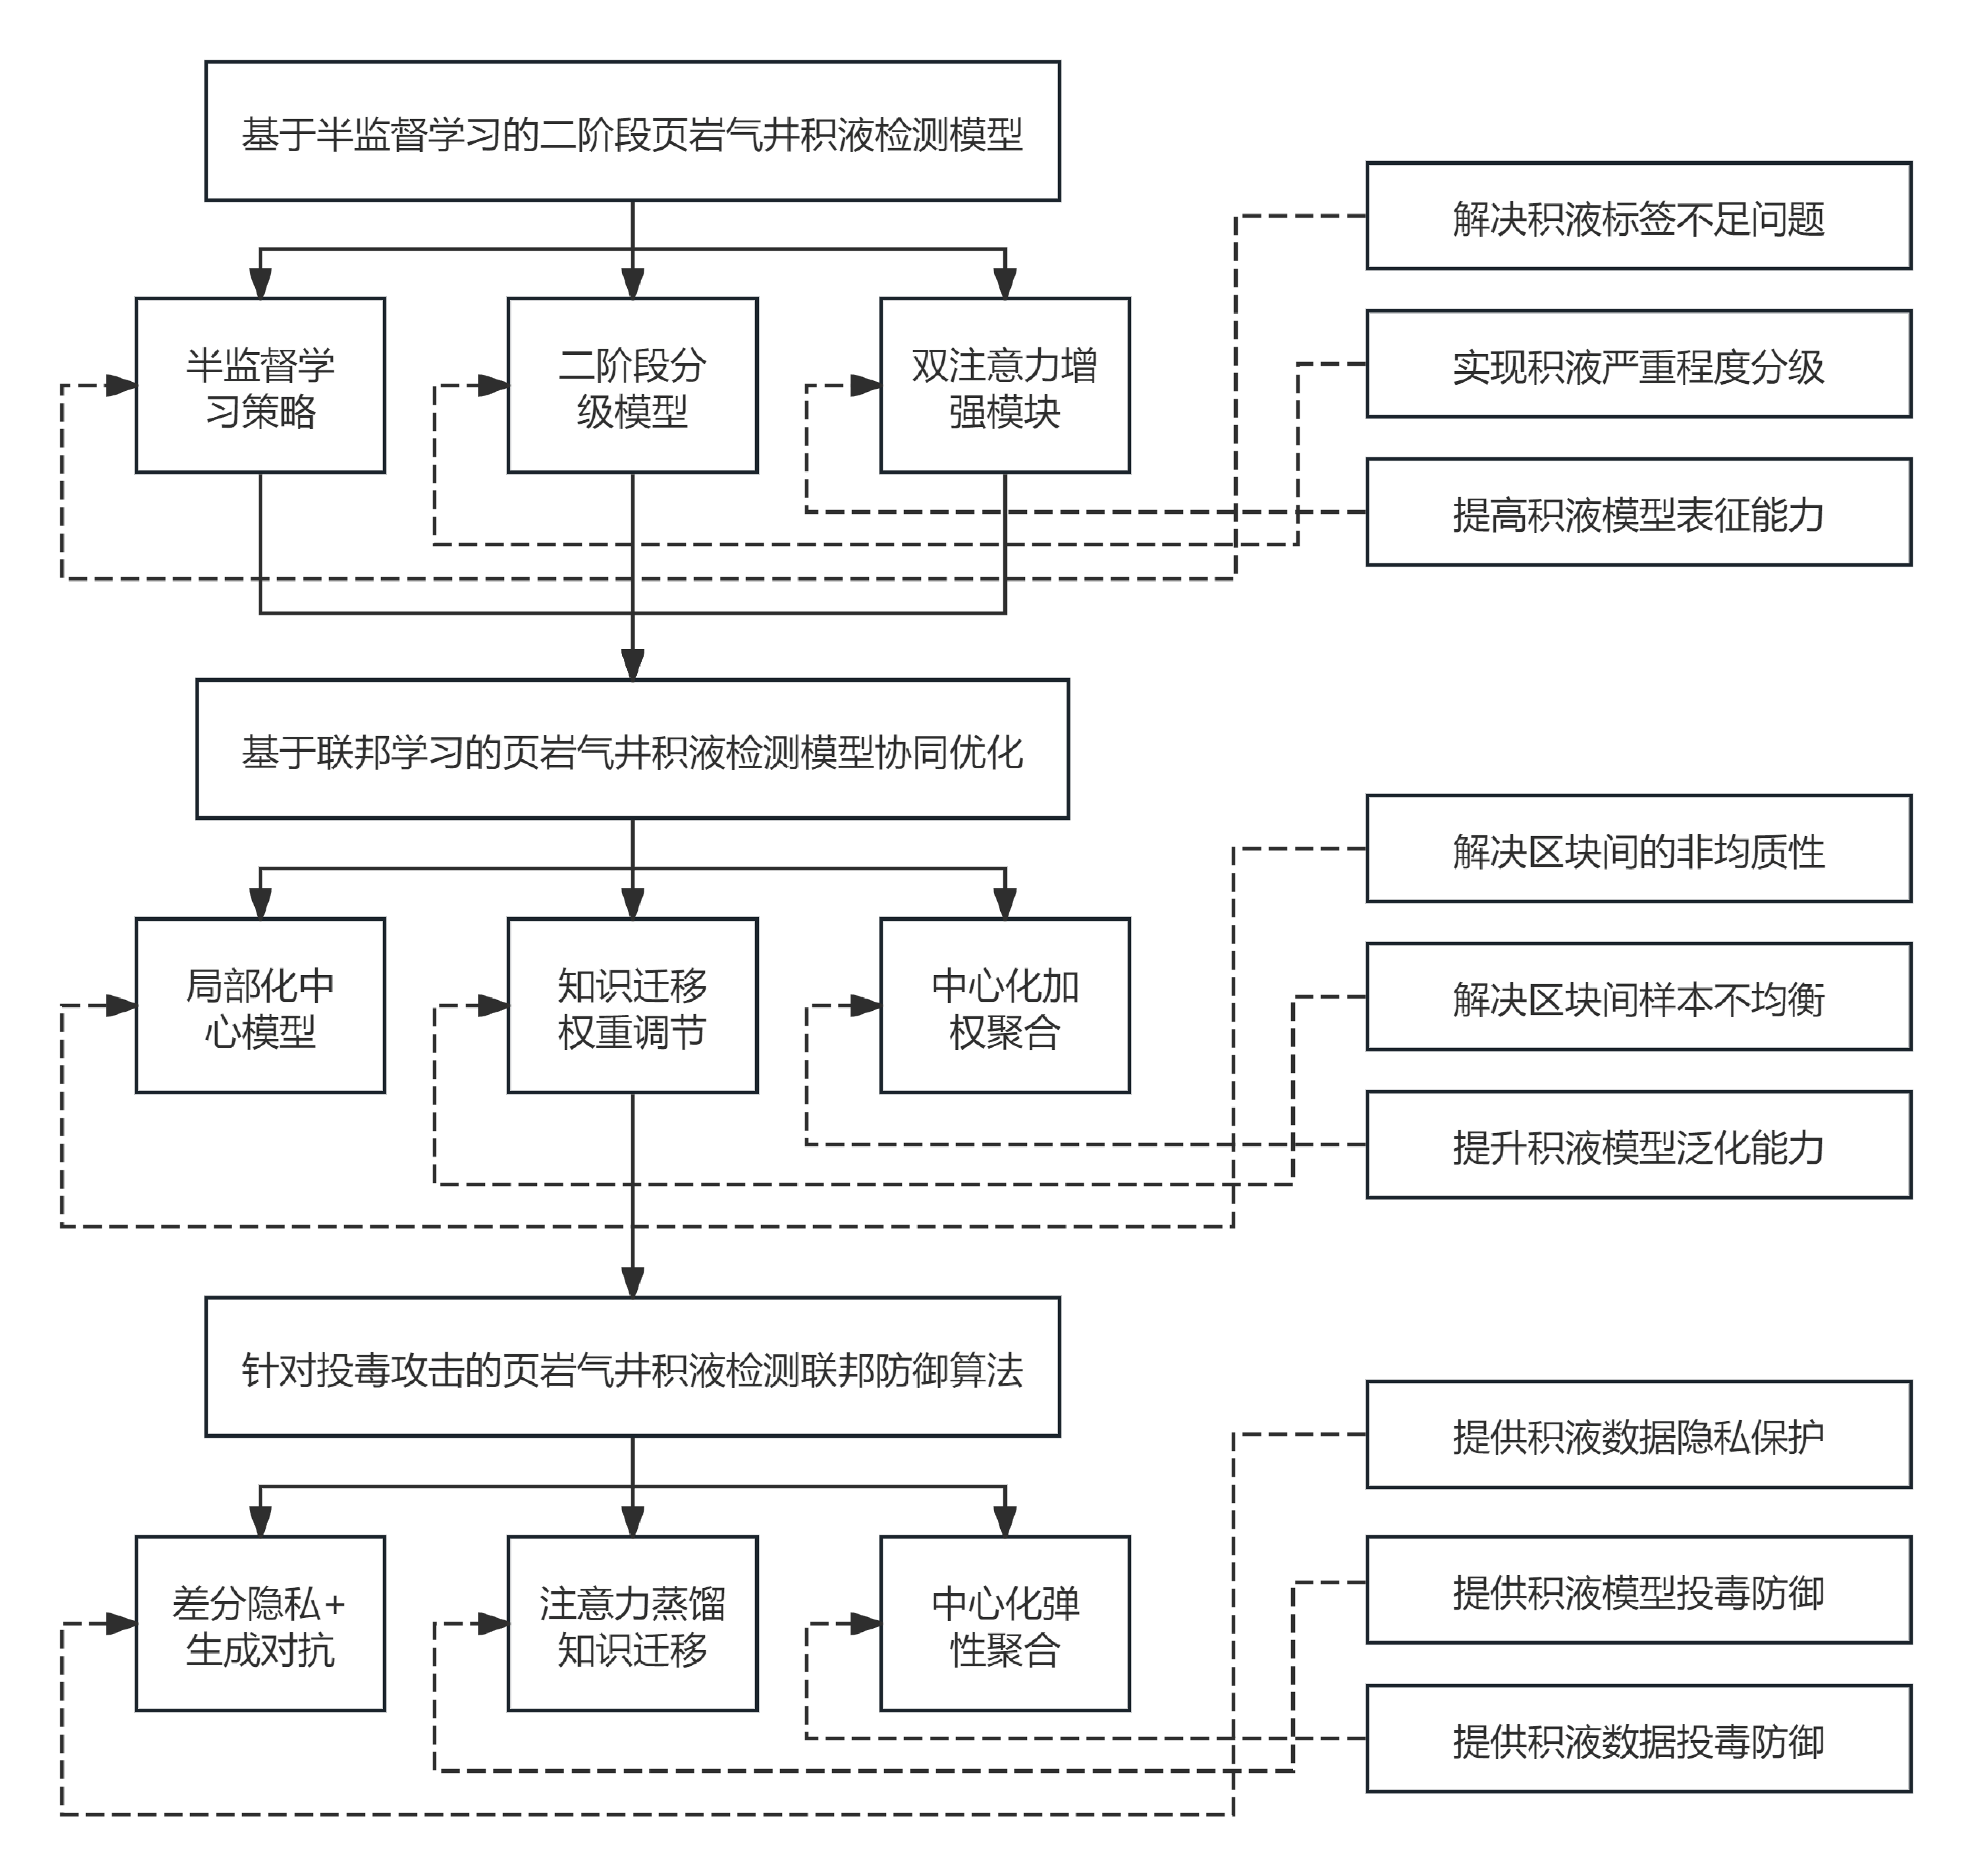
\includegraphics[width=0.8\linewidth]{fig/chapter1/图1-3.pdf}
	\caption{页岩气井积液检测场景下针对投毒攻击的联邦学习算法的研究架构}
	\label{fig:13}
\end{figure}
第一部分，我们提出了一种基于半监督学习的二阶段页岩气井积液检测模型。
该模型采用分段式设计：第一阶段通过检测积液是否存在，初步判断井筒的积液状态；
第二阶段在第一阶段的基础上，进一步对积液样本的严重程度进行分级。
这种分阶段的设计不仅提高了模型对积液状态的识别精度，还为排水措施的制定提供了量化依据。
在模型构建过程中，我们采用了半监督学习策略，充分利用少量标注数据与大量未标注数据进行训练。
该策略有效避免了大量标签制作所带来的高昂成本开销，同时借助标注数据为模型训练提供了必要的指导。
此外，我们还设计了一种双注意力增强模块，该模块强化了模型对积液特征的表征能力，
帮助模型实现更高的识别准确率。

第二部分，我们设计了一种基于联邦学习的页岩气井积液检测模型协同优化方法。
该方法为每个区块的积液检测模型设置了一个“局部化中心模型”。
该模型将从其他区块学习到的信息经过筛选，再传递到本地积液检测模型，
有效避免因区块间生产环境差异导致的模型性能下降。
此外，我们还设计了一种动态双向权重调节机制，
该机制包含中心化加权聚合算法和知识迁移权重调节算法两个部分。
中心化加权聚合算法以本地数据为参考标准，逐步整合其他区块的信息，
使积液模型在协同优化过程中保持一定个性化的同时逐步提升泛化能力。
知识迁移权重调节算法则能帮助样本量较少的新开发区块从协同优化训练中获取更多有利信息。

第三部分，我们针对投毒攻击的页岩气井积液检测联邦防御算法进行了深入研究。
在隐私保护方面，我们结合了差分隐私技术和生成对抗网络。在满足差分隐私加密强度的前提下，
降低了差分隐私技术对积液检测模型性能的负面影响。
在攻击防御方面，我们从模型投毒攻击和数据投毒攻击两个角度进行了研究。
针对数据投毒，我们在知识迁移权重调节算法的基础上，结合基于注意力蒸馏的防御算法，
形成了一种基于注意力蒸馏的知识迁移算法，
并验证了其在页岩气井积液检测模型协同优化场景下防御数据投毒攻击的有效性。
针对模型投毒，我们将拜占庭弹性聚合与中心化加权聚合相结合，
形成了一种中心化弹性聚合算法，增强了积液模型在面对恶意模型参数时的稳定性。

综上所述，本研究围绕页岩气井积液检测，
提出了一种融合半监督学习、联邦学习和隐私保护技术的综合解决方案。
通过半监督学习的二阶段检测模型，实现了积液状态的精准识别与分级。
在此基础上，借助联邦学习的协同优化，引入“局部化中心模型”和动态双向权重调节机制，
有效应对了生产环境的非均质性问题，提升了模型的泛化能力。
同时，结合差分隐私技术和生成对抗网络，优化隐私保护机制，
并通过基于注意力蒸馏的知识迁移算法和中心化弹性聚合算法，增强了模型对投毒攻击的防御能力。
该研究将积液检测的精度提升、模型优化与隐私安全防护有机结合，
为页岩气井的高效管理和安全运营提供了全面的技术支撑。

\subsection{主要创新}
本文创新点可总结为以下三点：

（1）通过半监督学习结合有监督和无监督学习的优势，解决了标签数据不足问题，
并采用二阶段设计进行积液检测和严重程度分级，辅以双注意力增强模块提高了模型的表征能力。

（2）通过为每个区块的积液检测模型设置“局部化中心模型”来避免生产环境非均质引起的模型偏向性。
并设计动态双向权重调节机制，帮助样本量较少的区块在协同优化过程中能够获得更多的关注。

（3）通过生成对抗网络+差分隐私技术在数据隐私保护强度与积液检测模型性能之间取得较好的平衡。
结合基于注意力蒸馏的知识迁移算法和中心化弹性聚合算法，
有效识别并防御积液检测模型在联邦学习训练过程中的投毒攻击。

\section{本文组织架构}
\textbf{第一章}：介绍论文的研究背景、国内外研究现状及本文的主要研究内容与创新。
阐述了当前井筒积液检测领域中主流的物理模型和数据驱动模型；
对联邦学习技术及其最新的投毒攻击与防御研究进行了综述。

\textbf{第二章}：介绍相关技术及理论。涉及传统井筒积液检测方法和基于数据驱动的检测方法；
对有监督、无监督和半监督学习策略进行了阐述；
重点介绍了联邦学习中的投毒攻击及其主流防御策略，分析了这些策略的优缺点。

\textbf{第三章}：介绍基于半监督学习的二阶段页岩气井积液检测模型。
详细说明了本研究所使用的数据集及数据预处理过程；
展示了二阶段井筒积液分级模型的具体结构，重点介绍了双注意力增强模块；
阐述了积液模型训练所采用的半监督学习流程。

\textbf{第四章}：介绍基于联邦学习的页岩气井积液检测模型协同优化方法。
详细展示了利用局部化中心模型思想完成页岩气井积液检测模型协同优化训练的整体流程，
重点介绍了动态双向权重调节机制，包括中心化加权聚合和知识迁移调节两个部分。

\textbf{第五章}：介绍针对投毒攻击的页岩气井积液检测联邦防御算法。
评估差分隐私+生成对抗网络方法的数据隐私保护强度及其对积液检测模型性能的影响；
评估基于注意力蒸馏的知识迁移算法在协同优化训练中对数据投毒攻击的防御效果；
评估中心化弹性聚合算法在协同优化训练中对模型投毒攻击的防御效果。

\textbf{第六章}：对全文进行总结与思考，并对未来研究方向进行展望。

